
%\UseRawInputEncoding
\documentclass{article}
\setcounter{secnumdepth}{0}
\usepackage[T1]{fontenc}
\usepackage[utf8]{inputenc}
%\usepackage[latin1]{inputenc}
%\usepackage[english, norsk]{babel}
\usepackage{filecontents}
\usepackage{tcolorbox}
\usepackage{url}
\usepackage{etoolbox}
\usepackage{framed}
\usepackage{framed, color}
\usepackage{xcolor}
\usepackage{mdframed}
\usepackage{float}
\usepackage{gensymb}
\usepackage{amsmath}

\definecolor{Black}{rgb}{0.0, 0.0, 0.0}

%Definer kode
\usepackage{listings}
\usepackage{color}
\definecolor{dkgreen}{rgb}{0,0.6,0}
\definecolor{gray}{rgb}{0.5,0.5,0.5}
\definecolor{mauve}{rgb}{0.58,0,0.82}

\lstset{frame=tb,
extendedchars = true,
texcl=true,
  language=C++,
  aboveskip=3mm,
  belowskip=3mm,
  showstringspaces=false,
  columns=flexible,
  basicstyle={\small\ttfamily},
  numbers=none,
  numberstyle=\tiny\color{gray},
  keywordstyle=\color{blue},
  commentstyle=\color{dkgreen},
  stringstyle=\color{mauve},
  breaklines=true,
  breakatwhitespace=true,
  tabsize=3
}

\usepackage[colorlinks]{hyperref}
\hypersetup{citecolor=Black}
\hypersetup{linkcolor=Black}
\hypersetup{urlcolor=Black}
\usepackage{cleveref}


\setlength{\parindent}{0em}
\setlength{\parskip}{1em}
%\renewcommand{\baselinestretch}{2.0}

%\renewcommand\thesubsection{\alph{subsection}}

\renewcommand{\figurename}{Figure}
\begin{document}
\author{Kent Odde}
\title{DCS3101\\Assignment 3}

\maketitle
\thispagestyle{empty}
\begin{center}
\includegraphics[width=\linewidth,height=0.2\textheight,keepaspectratio]{img/USN.png}
\end{center}
\newpage

\tableofcontents

\newpage

\section{Abstract}

This is my submission for the third compulsory assignment in DCS3101, Introduction to Cybersecurity.




\section{Q1}
\begin{tcolorbox}\textit{What are the advantages of firewalls?}\end{tcolorbox}
A firewall is a component, that functions as a check-point in a network, and its job is to monitor and regulate traffic passing through it.

The main use case and advantage of a firewall, is that we can protect a local trusted network against threats which might exist on another untrusted network.

When implemented, all traffic passing from network A to network B must pass through the firewall. The firewall may prohibit traffic it considers a threat. This decision has traditionally been based on a predefined rule set, but next-generation firewalls have much more sophisticated methods of identifying potential threats.

A strength of firewalls is their wide range of types suitable for different needs, and their capability for configuration. We can have an open firewall, where we define rules for what the firewall should filter out, or for a more conservative approach, we can have a firewall which filters all packages, and we white-list the traffic we do want.

We can filter traffic based the sender or receiver or by the contents of the packets, which can be used to protect specific hosts or specific ports. We can filter based on the types of application layer protocol the package contains, which can help us filter out spam mail etc. We can also use the TCP headers, so that an outgoing TCP packet on a port, will temporarily open the port for incoming packets, given that the TCP header contain the correct information.

There are also \textit{next-generation} firewalls, which can employ machine learning to be able to recognize unknown types of malicious traffic based on patterns.

As an added bonus of all this, we can also configure firewalls to log all traffic, which may be very handy for several reasons, but especially if we find out that our network has been compromised.


\newpage
\section{Q2}
\begin{tcolorbox}
  \textit{Comment if the following is true or false in the context of TLS - "The algorithms inside a session are negotiated between client and server." Justify your answer with an associated protocol diagram.}
\end{tcolorbox}
The statement in the question is \textbf{true}. Different clients and servers will have support for different encryption and MAC algorithms. Just like different people speak different languages. The goal of the negotiation is to find mutually supported algorithms, that are also recognized as secure enough by the current version of TLS.

However, negotiation is perhaps a strong word. If we look at subset of the TLS handshake protocol in figure \ref{TLS}, we can see that the client starts the conversation with a \textit{hello}.


\begin{figure}[H]
 \centering
  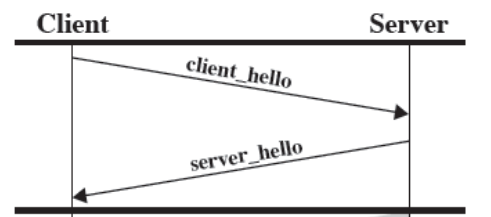
\includegraphics[width=200pt]{img/tlsHandshake.png}
 \caption{Part of the TLS handshake protocol diagram from lecture}
  \label{TLS}
 \end{figure}


This hello consists of information about the client, like what algorithms it has support for. One of the things the server then does, is to pick the strongest of these algorithms that it self supports. The server hello will then among other things, contain this decision.



\newpage
\section{Q3}
\begin{tcolorbox}
  \textit{It was discussed in the class about one particular attack on TLS. Discuss this attack and identify another attack that can impact TLS. Discuss briefly about the attack you have chosen for your answer.}
\end{tcolorbox}
The attack discussed in class was the exploitation of what has come to be known as the \textit{heartbleed bug}. This was a bug in the heartbeat protocol of TLS.

The heartbeat protocol, is a mechanism for letting the client check that the connection with the server is still active. The client would send a message asking for a distinct string as a reply, and the character length of this string. If the connection was still alive, the server would naturally send the requested string back.

However, it was discovered that if the number containing the length of the string was much higher than the actual length of the string, the server would in addition to the string send random content of its RAM. This was of course catastrophic, as a web-servers RAM is filled with a lot of information that can be exploited, like encryption keys and so on.


When it comes to other TLS vulnerabilities, there are plenty to choose from. They can be categorized into whether they arise from a flaw in the initial concept of TLS, the implementation, etc. Since heartbleed can be categorized as an implementation bug, I have chosen to write about a concept flaw.

\textbf{FREAK}

Freak is an acronym, and means \textit{Factoring RSA Export Keys}. In the 1990's computing power was scarce among the general public, and encryption did not have to be very strong to still be reckoned as secure. Previous to this, the American government had put a ban on the export of strong cryptographic technology, limiting applications meant for export to use RSA with a maximum of 512 bits. The upside to this was that the NSA was able to break these ciphers, but in essence, nobody else would.

However, throughout the 2000's computing power became more widespread. This meant that in essence, anybody would be able to break them. Luckily the cryptographic export laws were abolished in 2000, so by this time, most applications had moved on to stronger encryption.

The Freak attack however, made use of the fact that encryption of export grade were still available in a lot of applications and on a lot of servers. This allowed for a man in the middle, to trick clients to use weaker cryptographic schemes, and then easily decrypt the information sent.

This attack is no longer possible in TLS 1.3, as it no longer allows for a downgrade to the weaker protocols.

\newpage
\section{Q4}
\begin{tcolorbox}
  \textit{What are the differences between IDS and IPS? Discuss on classification/taxonomy of IDS and IPS.}
\end{tcolorbox}
In order to see the differences more easily, lets start with looking at the similarities.

Intrusion Detection Systems and Intrusion Prevention Systems are both constructs i the network infrastructure. They will analyze packets in the network, and in various ways check whether or not the packet is deemed as a threat. This is most commonly done by comparing the packet with the contents of a database, storing known malicious threats.

The main difference however is that while they both monitor the network and try to detect threats, an IPS will also prevent malicious packets from entering the internal network. In other words they live more in the domain of firewalls.

IDS can be separated into two main categories, based on the implementation:
\begin{itemize}
  \item{\textbf{Host Intrusion Detection}\\Individual host implementation. Dependent on the logs within the host. May take up a lot of resources on the host.}
  \item{\textbf{Network Intrusion Detection System}\\Monitors traffic on the network, to and from all hosts. It is easy to implement.}
\end{itemize}

However, we can also categorize them based on their method of threat detection:
\begin{itemize}
  \item{\textbf{Signature-based Intrusion Detection Systems}\\Looks for specific bit sequences in the packet payload, which has been flagged as a possible threat. Can not detect new threats.}
  \item{\textbf{Anomaly-based Intrusion Detection Systems}\\The system uses training data, to learn what is deemed as \textit{normal} traffic, and then it looks for packets which deviate from the norm to a certain degree.}
\end{itemize}

As far as I could find, IPS is also classified by the same categories as IDS, as it of course has a detection system within. I could unfortunately not find any categories or differences of how the actual prevention is done.

\newpage
\section{Q5}
\begin{tcolorbox}
  \textit{Biometrics - What are the key factors for choosing a biometric modality (e.g., face, fingerprint, iris, etc)?}
\end{tcolorbox}
As with every other choice, the decision of which biometric modality to use depends on the particular use case.

If one is dependent on extremely robust security, the best choice will differ than if they key factor was user convenience and security was second priority.

The metrics of modalities as mentioned in the lectures are great ways for making this decision:

\begin{itemize}
  \item{Failure-to-Capture Rate}
  \item{Failure-to-Extract Rate}
  \item{Failure-to-Enrol Rate}
  \item{Failure to Acquire Rate}
  \item{False-Match-Rate}
  \item{False-Non-Match Rate}
\end{itemize}
The first four points are very important if the goal is user convenience, as a lot of failures of creating and storing a template will result in irritation. However, if the key goal is security, high numbers here may be acceptable.

The two last points will be a trade off between usability and security. If the false match rate is virtually zero, the false non match rate will probably be higher. As no system is perfect, this will be a choice depending on how critical security is.


\newpage
\section{Q6}
\begin{tcolorbox}
  \textit{What kind of attacks are possible on face biometric systems?}
\end{tcolorbox}

Face biometric systems may be susceptible to several attacks, based on the sophistication of the implementation.

The most obvious one is of course just threatening the person to which a face belongs, to unlock the system. However, this sort of attack is not very sophisticated, carries great risk, and is quite rare.

Among the more realistic attacks, they all revolve around simulating the face in some way. These are often called presentation attacks.

You can have a photograph of a face, a video of a face or various types of masks.

Whether or not these work, depend on the implementation. To combat them one may use sensors or 3D-cameras to make sure that there is in fact a person present. One may also use particular expressions or movements in the face when storing the template.

There are also more classical attacks, that apply for all sorts of security, where one tries to access the system, and manipulate the template database or weaken the match acceptance criteria.

\newpage
%Referanse
%\section{Referanser}

\nocite{*}
\bibliographystyle{plain}
\bibliography{ref}

\addcontentsline{toc}{section}{References}

\end{document}
